\chapter{Background}
\label{chapter:background}
\minitoc

Content sharing is currently a universal concern among computer users and has recently become an important requirement for mobile devices. Indeed, thanks to the efficient wireless connectivity offered by mobile devices, users are frequently brought to locate and share content of interest (photos, videos, etc) with other members of the same spontaneous community. With current technologies, users are mainly using point-to-point basic connections, which can be considered as an efficient solution when the number of users interested in the sharing session is very small and that there is no risk of connexion disruption. However, even with a guaranteed wireless connection and in the case of a large community (for example, mobile device users assisting to a conference and willing to share some papers), one is facing the following problem: increasing the number of parallel point-to-point communications may decrease the global Ad Hoc network capacity, while increasing dramatically the download time. The multi-hop point-to-point communication over long paths is also a serious issue. Therefore, there is a strong need to organize the communication overlay among devices in a way to distribute fairly the burden of content sharing among the set of participants while aiming to decrease the global download time. P2P file sharing solutions are good candidates for such infra-structureless networks (MANET) as they are based on multi-sourcing which balances resource consumption among users and reduces the dependency on any central entity. But unfortunately, P2P content sharing applications developed for the Internet cannot directly be plugged and used into mobile devices. Indeed, on one hand, these solutions are not adapted to the constraints of multi-hop wireless networks. For example, it is known that in a resource constrained environment, the choice of the users to whom to connect cannot be done independently of information on the underlying dynamic topology. Moreover, centralized users management approaches like the centralized tracker used in BitTorrent do not perform well in such environment as the tracker can be either far away or even invisible by some users because of disconnections. Furthermore, computer users rely on Internet search engines and dedicated desktop applications to look for the content they are willing to share. This approach becomes obsolete in the case of a spontaneous MANET based community and thus, a dedicated distributed content discovery approach must be provided. 

Then, if we consider a more general/challenging mobile environment where the topology is unstable and users' contact can be disrupted frequently (for example, mobile devices users moving in the street), users cannot rely any more on the content dissemination systems proposed for conventional MANETs~\cite{BitHoc}~\cite{BlueTorrent}. Indeed, the later ones are built based on the assumption that the network path are almost stable and that content providers and content consumers are connected to the same part of the network at the same time. Therefore, they are not suitable for disruption tolerant environment. From this perspective and to allow some services to operate even under
these challenging conditions, researchers have proposed a new networking paradigm, often referred to as Disruption Tolerant Networking, based on the store-carry-and-forward routing principle. Devices there, rather than dropping a session (and respectively packets) when no forwarding opportunity is available, store and carry
content until new communication opportunities arise. 

This chapter describes the background behind our work. At first hand, we discuss content sharing challenges in MANETs. We focus on P2P content sharing solutions and we give an overview of \emph{BitHoc}, the P2P open-source standalone content sharing solution that we proposed and developed for MANETs. We then discuss the reasons that could prevent users from adopting BitHoc as a content dissemination solution in the context of a disruption tolerant environment. 

At second hand, we give an overview of already existing solutions for content sharing in a disruption tolerant environment (both point-to-point content routing and point to multi-point routing protocols), we detail the limitations of the different proposed approaches and we discuss those we are able to overcome through the solutions we are proposing in this thesis.

\section{Content sharing in MANETs}

\subsection{MANETs}

Nowadays, wireless networks have become more and more popular as they are easily deployable. These networks play a crucial role among computer networks, since they offer solutions to support mobility and essential services without the need of any installed infrastructure. Wireless networks can be classified into two categories: infrastructure wireless networks using generally the cellular communication model and wireless networks without any infrastructure called mobile ad hoc networks (shortly MANET). An ad hoc network consists of a set of mobile entities (computers, PDAs, mobile phones, etc) moving in any environment and using wireless interfaces as communication links. The main sources of problems encountered in such networks are bandwidth limitation, energy limitation and the pseudo-random mobility of nodes. Here are more details about the characteristics of mobile ad hoc networks:
\begin{itemize}
\item{A dynamic topology due to the mobility of nodes and churn. The network can even be partitioned into separate islands when nodes go out of the wireless range of each others.}
\item{A limited bandwidth that diminishes dramatically with the size of the exchanged information. Apart from being scarce, this bandwidth is shared among the set of nodes. In fact, nodes in the transmission rage of each other cannot send packets simultaneously because of radio interferences.  Furthermore, sending packets to far away destinations steals bandwidth in intermediate nodes acting as routers.} 
\item{Nodes are constrained energetically and their autonomy is dependent on their battery loads. Hence, they must minimize packet transmissions to limit energy consumption if they want to increase their lifetime.}
\item{Wireless channels can be subject to severe errors and losses due to fading and collisions and other exterior interferences.}
\end{itemize}

Despite of these constraints, wireless ad hoc networks have the particularity of being self-constructed, self-organized and self-configurable without needing any fixed infrastructure. Wireless ad hoc networks are traditionally used in military applications, emergency services (earthquakes, fires, flooding, etc) and sensor networks (climatology, meteorology, detecting earth movements, etc). Nevertheless, the tremendous increase in computing abilities of devices and their network capacities has encouraged users to connect to each other to form communities in order to share their experience (social networks, content sharing, video streaming, etc). Hence, new applications already popular in the Internet such as Instant Messaging, file sharing and social networks are being migrated for the wireless ad hoc environment.

To run the applications described above, one need to ensure the connectivity of the network and the routing of packets. The routing algorithm is a strategy that ensures the connectivity between each couple of nodes at any moment. If the nodes are not in range of each others, the connectivity passes by other nodes which serve as relay or router. This strategy must take into consideration the changes in the network topology and other important characteristics such as the bandwidth, the number of links, the limitation of energy, etc. Considering this challenge, many routing protocols have emerged to answer different objectives and solve different problems.  In the following paragraphs, we present the main routing solutions for wireless ad hoc networks using different current strategies. There are many criteria to design and classify routing protocols for wireless ad hoc networks: how nodes exchange routing information, when and how paths are computed, etc. Hence, three large categories of routing protocols~\cite{Royer:RoutingSurvey,Broch:98performance} can be distinguished:

\begin{itemize}
\item{\textbf{Proactive protocols:} Paths are pre-established based on a periodic exchange of routing tables.}
\item{\textbf{Reactive protocols:} Paths are found by the network on-demand. Nodes request each other in order to detect a possible path to the destination.}
\item{\textbf{Hybrid protocols:} They combine the proactive and reactive approaches to profit of their advantages and reduce their drawbacks.}
\end{itemize}

\subsection{MANETs and the P2P paradigm}

Recently, P2P systems have gained a lot of popularity since users profit from resources offered by thousands of other users. In fact, such systems are composed of dynamic sets of nodes connected to the Internet and were initially designed to ensure file sharing. Nowadays, the P2P paradigm emerges as a general philosophy for constructing large scale services and distributed applications in the Internet. Hence, one can define without loss of generality P2P systems as being self-organizing and distributed systems. The nodes of a P2P network play symmetric roles. Indeed, they are both clients and servers. However, some of these nodes can be potentially non reliable and can show different levels of collaboration. Furthermore, P2P networks are a good example of Overlay networks. An Overlay network is an abstraction of the physical network at the application level. Consequently, an ideal P2P overlay network must be self-organized and decentralized and must hide the diversity and heterogeneity of its nodes.

Although they are used independently, P2P overlay networks and MANETs share many common characteristics like self-organization and decentralization. This is due to the common nature of their distributed components. On one hand, a P2P Overlay network is composed of a dynamic set of nodes connected through the Internet. On the other hand, a mobile ad hoc network is composed of mobile nodes communicating together with multi-hop wireless links. These common characteristics yield other similarities:

\begin{itemize}
\item{Both networks have flat topologies with frequent changes caused by nodes that join and leave the network. For wireless ad hoc networks, the physical mobility of nodes also causes changes in the topology.}
\item{Both networks establish connections hop by hop. Multi-hop connections in P2P networks are typically constructed thanks to TCP connections without physical limitation. However, in MANETs, multi-hop wireless connections are limited by the range of radio transmission.}
\end{itemize}

The common characteristics between P2P Overlay networks and MANETs show that these two types of networks share the same main challenge of ensuring the connectivity in a dynamic and decentralized environment. Hence, there is a synergy between the two networks in terms of their goals and the design principles of their algorithms and protocols.  These algorithms and protocols must consider the dynamic nature of the network topology due to churn and mobility. The similarities between P2P networks and MANETs and the design concerns shared among them brought to life a new research direction in computer networks, which profits from the synergy existing between P2P overlay networks and mobile ad hoc networks to design better routing protocols and applications.

In the following section, we present BitHoc~\cite{BitHoc, BitHocWeb}, the architecture we proposed for content sharing in MANETs and  will answer the following important questions:

\begin{itemize}
\item{Can one profit from the similarity existing between the architectures of P2P networks and MANETs to design protocols and applications for content sharing over MANETs?}
\item{How to adapt P2P overlays to mobile ad hoc networks?}
\end{itemize}

\subsection{BitHoc: A P2P Content Sharing Solution for MANETs}

MANETs are an adequate field for content sharing among communities of users. Indeed, users can connect to each other in order to share data and multimedia files without being connected to any infrastructure network. To ensure this connection at the data transfer layer, they need to agree on a content distribution protocol. The classical transfer methods namely the client/server and the application level multicast methods are not the most suitable for wireless ad hoc network for many reasons. First, they yield important overhead on the underlying wireless network as their communication graph is not designed for networks where resources are limited and shared. Moreover, the load of data transfer is not fairly distributed among the set of nodes since the nodes that are nearer to the source of the content will send more packets than other nodes that are far from it. The target of these methods is to have a hierarchy of nodes where some of them sacrifices some of their capacities to serve others without any incentives built in the protocol. 
Hence, a suitable content sharing paradigm must minimize the consumption of network resources and must divide the burden of sharing data equally among the set of nodes by thinking about the topology of the network and giving enough incentives for fair sharing. Furthermore, it must maximize the global capacity of the system by using the ability to have parallel communications in different areas of muti-hop wireless networks.

Having these goals in mind and starting from the well known P2P file sharing paradigm in the Internet where a peer uploads to other peers as much as it receives, we adapt BitHoc to the constraints and the nature of wireless ad hoc networks. Our objective is to come up with a general, stand-alone and efficient solution for content sharing in wireless ad hoc networks that is inspired of the BitTorrent protocol~\cite{RefBT}. The construction of the content sharing overlay in the Internet version of BitTorrent is done independently of the underlying topology and can engender a big routing overhead in a wireless ad hoc environment.

In the remaining of this section, we describe our solution for content sharing in MANETs, BitHoc~\cite{BitHoc, BitHocWeb}. The latter provide solutions to the following problems:

\begin{itemize}
\item{In the classical Internet version of BitTorrent \cite{RefBT}, peers periodically contact a central rendezvous point called Tracker to obtain fresh information about the peers interested in a specific content and to update their information on the progress of the download. This membership information is dynamic since peers can join and leave the content sharing overlay (called torrent) at any time during the session. Because of the inappropriateness and the large overhead of client/server architectures in wireless ad hoc networks, it is important to introduce a distributed Tracker-less solution to manage the membership of the sharing session. The BitHoc tracker component of our architecture is designed for this purpose and is inspired from the membership management protocol we presented in details in~\cite{BitHoc}.}
\item{The classical Internet version of BitTorrent \cite{RefBT} supposes that the cost of sending data packets to peers is in somehow independent of their locations. In an ad hoc network, performance metrics like achievable throughput, delay, and energy consumption strongly depend on the number of hops to the peer node. So, it is clearly suboptimal and even unrealistic to deal with peers without considering the underlying topology. Furthermore, when applying the classical BitTorrent incentives in a wireless multi-hop network, nodes fail to reciprocate data fairly among them. The content dissemination scheme is close to a wave transferring data from the initial seed to the farthest peers. Through new peer selection and content piece scheduling strategies, our solution is topology-aware and ensures fair sharing. These strategies are described in details in~\cite{BitHoc}.}
\item{To join a sharing session, a user should find and download the Torrent file related to that session. In the Internet, peers usually find their torrent files by the help of search engines which mainly look for the files in different central servers. This method does not apply in a mobile ad hoc environment as MANETs. The BitHoc search engine overcomes this challenge by maintaining a distributed Torrent file database thanks to the overlay constructed by the BitHoc Tracker.}
\end{itemize}

\subsubsection{Architecture of BitHoc}
\label{secarchitecture}

Figure \ref{figarch} depicts the principal components of this architecture and the interactions between them. We illustrate these interactions through three typical usage scenarios:

\begin{figure}[!h]
  \begin{center}
    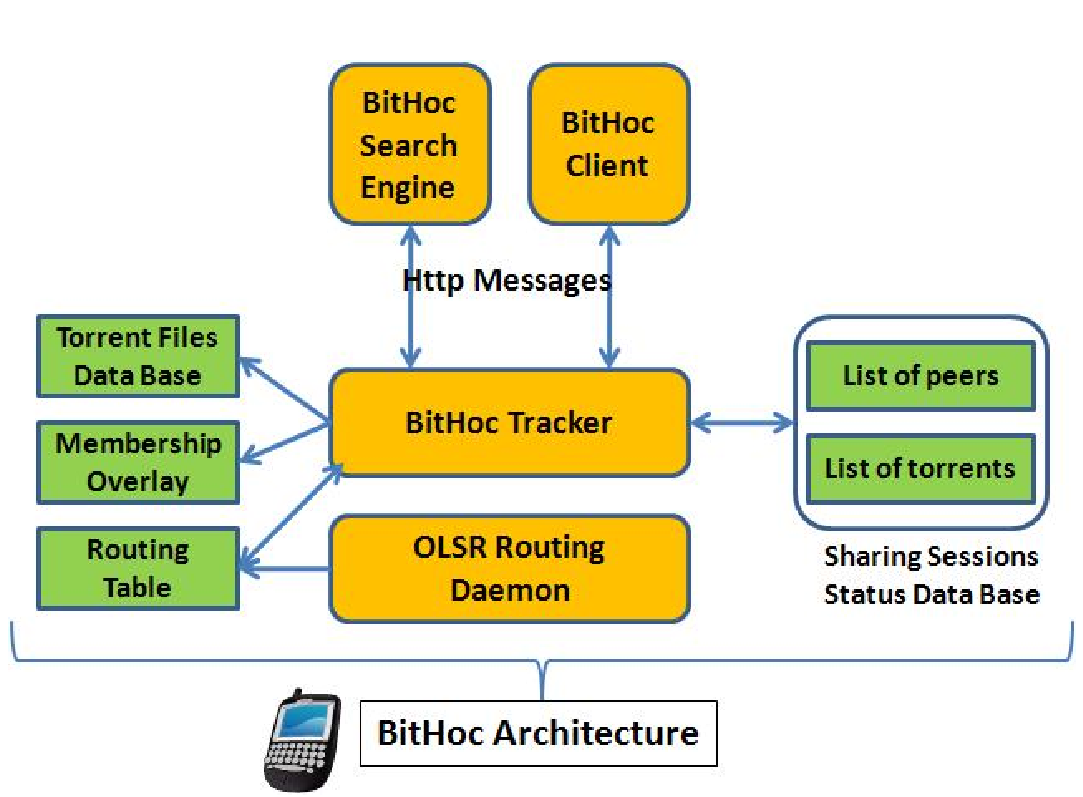
\includegraphics[width=0.7\textwidth]{Chapitre2/architecture.png}
  \end{center}
  \caption{Architecture of BitHoc}
  \label{figarch}
\end{figure}

\paragraph{Content publishing and discovery}

A user willing to share some content with the members of his community needs to indicate to the BitHoc client the location of the content in the mobile device file system. First, the client creates a meta-info file (Torrent file) that identifies in a unique manner a sharing session for this specific content. After that, the user publishes (locally) the new torrent file and a short text description of the related content using the BitHoc Search Engine service, which will update the local Torrent file database maintained in the underlying BitHoc Tacker via HTTP messages. A remote user, willing to share the same content, has to use the BitHoc search engine to find and download the Torrent file. He specifies for that the name of the content or some keywords related to its description. The request is sent via HTTP messages to its local tracker which looks for the closest match in its local database. If there are no matches, it forwards the HTTP request to the other trackers in the discovery overlay. Then, it presents the received results through an ergonomic user interface (see Figure \ref{Figsearchengine}). Based on the details of received answers (fitness to the search, number of peers involved in the sharing session, number of seeders, and number of lechers, etc), the user can choose the torrent file to download, then start sharing the content using the BitHoc Client.

\begin{figure}[!h]
  \begin{center}
    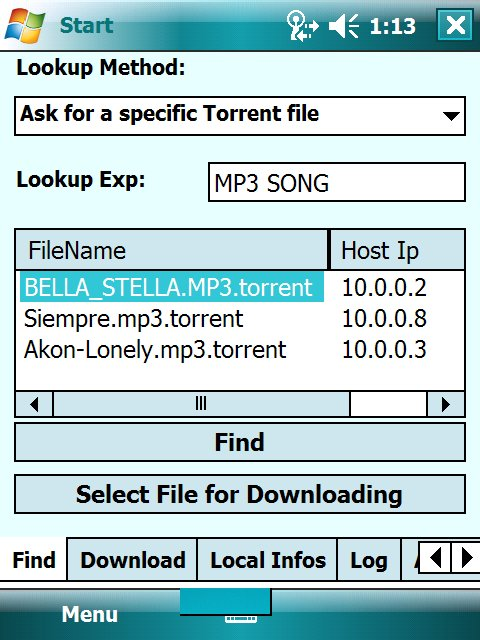
\includegraphics[width=2in,height=3in]{Chapitre2/searchengine.png}
  \end{center}
  \caption{Search Engine screen shot}
  \label{Figsearchengine}
\end{figure}

\paragraph{Membership management}

When a peer wants to join or leave the sharing session, the BitHoc client informs the BitHoc Tracker about this event using a specific HTTP message. This local agent disseminates this modification to the other BitHoc Tracker agents in other nodes in order to update their knowledge about the global membership information. The communications between Tracker agents are established in an event-driven fashion and use HTTP messages. Each tracker holds a HTTP server accepting HTTP requests from other agents and from the local BitTorrent client. The BitHoc Tracker component receives from the routing daemon up-to-date routing entries. In our testbed, the dynamics of the Ad-Hoc network are captured by the OLSR routing protocol \cite{OLSR}. Each time the number of hops toward a given peer changes, the routing daemon fires an event, which will be caught by the BitHoc Tracker and forwarded internally to the BitHoc client. This way we are sure the peer selection strategy always uses the updated number of hops to other peers. The parameters of the communications among tracker agents like HTTP listening ports and IP addresses can easily be configured by users via an ergonomic GUI. In addition to these functionalities, the BitHoc Tracker allows the user to monitor in real-time the status of the overlay (Contents it shares, members of the session, current topology of the Ad-Hoc network). He can even decide to keep traces about all the events in a file. For this, he just needs to activate the tracing option provided by the application.

\paragraph{Content sharing}

Before starting a new sharing session, the user can choose between two versions of BitTorrent algorithms: The classical version \cite{RefBT} and our version adapted to mobile Ad-Hoc networks described in~\cite{BitHoc}. The BitHoc client offers a Wizard allowing the user to configure the parameters of BitTorrent (communication ports, choking slot duration, minimum and maximum number of peers, etc). Once the torrent file is obtained, the BitHoc client can start the sharing session where it can either play the role of a leecher or a seed. It contacts periodically the local BitHoc tracker to get the current list of members of the same content sharing session (torrent). Using this list and the routing table, it manages the connections with the interested peers. Briefly a client implementing our algorithms exchanges pieces with close peers and only seeds distribute pieces across the network. Note that we allow the user to pause or resume the download while conserving the session context. He can also monitor in real time the status of the session (downloaded bytes, uploaded bytes, numbers of leechers, number of seeders, elapsed time, etc). Furthermore, the BitHoc client keeps in a log file statistics on the content sharing session and provides different levels of event traces. It also manages the storage of the downloaded contents and their classification. Figure \ref{Figclient} shows a screen-shot of the BitHoc client.

\begin{figure}[!h]
  \begin{center}
    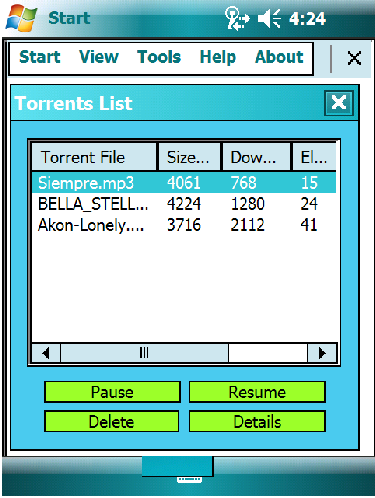
\includegraphics[width=2in,height=3in]{Chapitre2/contentsharing.png}
  \end{center}
  \caption{BitHoc Client screen shot}
  \label{Figclient}
\end{figure}

\subsubsection{Experimentation and results}
\label{sectest}

\paragraph{Test-bed description}

Our wireless Ad-Hoc network experimental environment consists of 14 mobile devices including 7 PDAs (HP iPAQ 214) and 7 smart-phones (HP iPAQ 614c). Each hand-held is equipped with an IEEE802.11b wireless card. The characteristics of the two types of devices are detailed in Table \ref{tabcarac}. The Ad-Hoc connectivity is maintained thanks to OLSR daemons run by the different devices. In our experiments, we constructed several network topologies containing a maximum of 6 hops. The objective of the realized swarm was to download a 4 MB MP-3 content. All PDAs were supposed to participate to the sharing of the file. The original seed of the content was chosen randomly among the set of the 14 PDAs.

\begin{table}[!h]
\center
\label{tabcarac}
\caption{Characteristics of mobile hand-held(s)}
\begin{tabular}{|l|c|c|}
  \hline
   & \textbf{PDA} & \textbf{Smart-phone} \\
  \hline
  \textbf{Name} & HP iPAQ 214 & HP iPAQ 614c\\
\hline
  \textbf{Processor speed} & 624 MHz & 520 MHz \\
  \hline
\textbf{RAM} & 128 MB & 128 MB \\
  \hline
\textbf{Operating system} & Windows Mobile 6 & Windows Mobile 6 \\
  \hline
\end{tabular}
\end{table}

\paragraph{Experimentation results}

\begin{figure}[!h]
  \begin{center}
    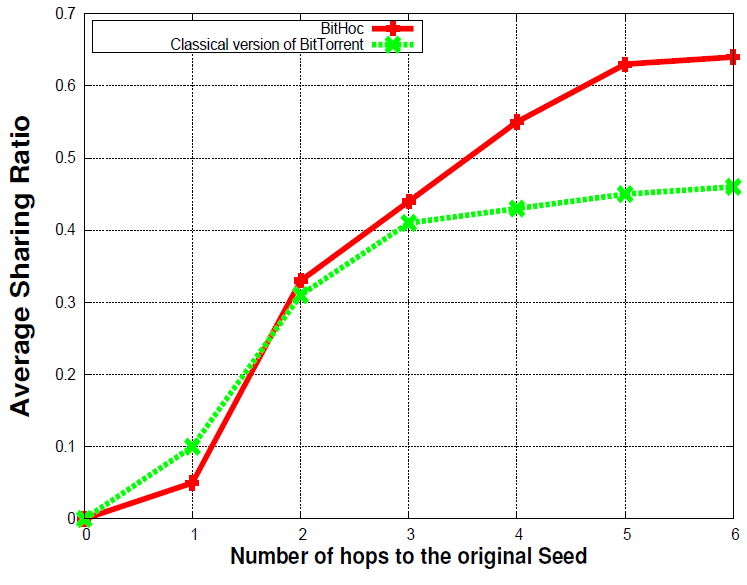
\includegraphics[width=3in,height=2.2in]{Chapitre2/sharingratio.png}
  \end{center}
  \caption{Sharing ratio}
  \label{figsharing}
\end{figure}

\begin{figure}[!h]
  \begin{center}
    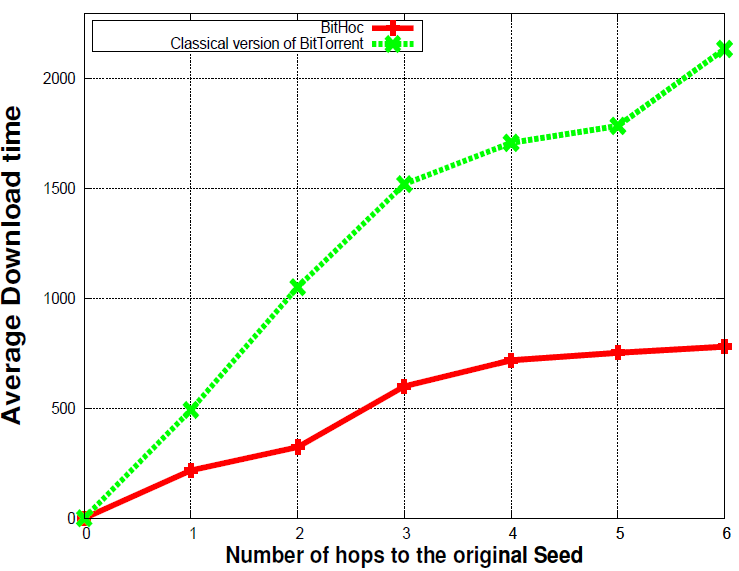
\includegraphics[width=3in,height=2.2in]{Chapitre2/downloadtime.png}
  \end{center}
  \caption{Download time}
  \label{FigDownloadtime}
\end{figure}

The metrics tracked during our experiments are the download time and the average sharing ratio of nodes. We define $R_{h}$ as the sharing ratio of peers located at $h$ hops from the original seed. It measures the level of reciprocity between downloads and uploads. In the ideal case, the ratio should be close to $1$. The two versions of BitTorrent (The legacy one and ours) have been tested and the results are presented in Figures \ref{figsharing} and \ref{FigDownloadtime}. Figure \ref{figsharing} shows a dramatic increase of sharing opportunities when our adapted version is deployed. The routing overhead generated by the classical version makes any gain obtained by important diversification of pieces negligible. Our method finds the good equilibrium between sharing and diversification. Figure \ref{FigDownloadtime} shows that BitHoc outperforms the classical version of BitTorrent in terms of download time. It is in accordance with our research results presented in~\cite{BitHocWeb}. More information about our experiments and our GPL licensed open-source code can be found on the BitHoc web site \cite{BitHocWeb}.

\subsubsection{BitHoc limitations with respect to a disruption prone environment}
\label{BitHoc:limitations}

We should note that BitHoc is built based on the assumptions that the network path are almost stable and that content providers and content consumers are connected to the same part of the network at the same time. Indeed, as described in Figure~\ref{figarch}, BitHoc relies on the routing table built and maintained by the OLSR MANET routing protocol towards maintaining the sharing sessions membership overlay and in order to deliver messages to peers at more than one hop. Therefore, BitHoc is not suitable solution for content dissemination in a disruption tolerant environment. 

\section{Content sharing in Disruption Tolerant Networks}

\subsection{Disruption Tolerant Networks}

Delay and disruption tolerant networks (DTNs) are a new class of wireless networks that seek to address the networking issues in mobile or challenging environments that lack
continuous network connectivity. DTNs have emerged recently and are continuing to gain extensive efforts from the networking research community~\cite{Bundle,fall03,dtnrg}. In the literature, these networks are found under different terminologies such as sparse mobile ad hoc networks, extreme wireless networks, or under another commonly used term intermittently connected networks. Basically, DTNs appear in areas where the network spans over large distances with low node density and/or with high node mobility. DTNs might appear also due to short radio range, power saving mechanism at the nodes, or nodes failure. Examples of such networking scenarios include, but are not limited to :

\begin{itemize}
\item{Vehicular networks, e.g.~\cite{Levine:MaxProp, DriveThru}. In~\cite{DriveThru}, the authors propose the Drive-thru Internet architecture where the objective is to provide network and Internet connectivity
to mobile users in vehicles. The network is constituted by hot spots that are placed along the roads providing thus intermittent connectivity to the users that can
connect within proximity. In~\cite{Levine:MaxProp}, Burgess et al. introduce UMass DieselNet which is a network made of 30 buses equipped with 802.11b wireless interfaces and GPS devices. The objective of the network is to provide real DTN testbed for experimental and research studies. The buses move on regular trajectories inside the UMass Amherst campus and surrounding areas. When two buses pass nearby, they transfer data to each other. Additionally, buses can connect to open wireless access points
along the roads.}
\item{Mobile sensor networks for environmental monitoring, e.g.~\cite{zebranet02,WirelessInfostation}. Zebranet~\cite{zebranet02} is a wireless networking architecture designed to support wildlife tracking for biology research. In ZebraNet, the network is constituted by sensor collars that are attached to zebras, which log movement patterns of the zebras, and by base stations that are mounted on cars which move around sporadically. When two zebras meet, the corresponding sensors exchange collected data for a potential data delivery back to base-stations. Another similar biological acquisition system has been proposed in~\cite{WirelessInfostation}, where the network is made of a set of sensors attached to whales and a set of fixed info-stations that act as collecting nodes.}
\item{Communication between rural zones in developing countries, e.g.~\cite{Brewer:DTNdeveloping}. Examples include DakNet~\cite{Brewer:DTNdeveloping} which is a wireless ad hoc network that has the capacity to provide asynchronous Internet access to remote rural residents using motorcycles and buses to carry users email and web search messages.}
\item{Deep space networks such as the Inter-planetary network (IPN)~\cite{interplanetary03}. The interplanetary network is a network of regional Internet networks. A region is an area where the characteristics of communication are the same. An example of regions includes the terrestrial Internet as a region or a ground-to-orbit region. IPN aims to achieve end-
to-end communication through multiple regions in a disconnected, variable-delay environments.}
\item{Challenged networks such as disaster healing networks after natural disaster, travel information and advertisements dissemination systems in large cities using local transport systems, military ad hoc networks where disconnection occurs because of the war or for security reasons where some links need to be shut down from time to time.}
\end{itemize}

Generally speaking, DTNs are wireless networks that do not conform to Internet or to traditional multi-hop and ad hoc wireless networks underlying structures and assumptions.
In particular, they are characterized mainly by the following specific features~\cite{fall03, DTNTutorial}:

\begin{itemize}
\item{Intermittent connectivity where an end-to-end path between a given source-destination pair does not exist most of the time. Path disconnections are frequent and arise from
two main factors, namely motion and/or limited power at the nodes. Disconnections due to motion can arise when one or both nodes at the end of a communication link move, or due to some intervening objects or signals that obstruct the communication. These disconnections can be predicted, for instance when the nodes move away
according to a predetermined schedule, or opportunistic for instance according to random walk of the nodes. Disconnections that are due to power outage result
commonly from some power saving mechanisms at the wireless devices, e.g. case of sensor networks. The latter disconnections are often predictable.}
\item{Nodes have low power capabilities and limited resources. In many DTNs, nodes are generally battery powered and/or deployed in areas lacking power infrastructure. In
some other situations, nodes have limited memory and/or processing capabilities.}
\item{Large delays which are basically due to long queuing times resulting from frequent disconnections, or from low data rate at the devices.}
\end{itemize}

\subsection{Content Sharing in Disruption Tolerant Networks}

Due to frequent disconnections in DTNs, instantaneous end-to-end routes do not exist, and hence most of the traditional Internet and/or mobile ad hoc content routing protocols fail~\cite{Fall:DTNrouting}. However, end-to-end routes may exist over time if the nodes can take advantage of their mobility by exchanging and carrying other nodes messages upon meetings, and by delivering them afterward to their corresponding destinations. The latter concept has given rise to a novel routing paradigm in these networks called the \emph{carry-and-forward approach}, in which intermediate nodes serve as relays for each other. Thus, the term "mobility-assisted routing approach" that is used in conjunction to describe these schemes.

Unfortunately, these techniques result in high latency, since packets need to be carried for long time periods before being delivered. When the delivery latency is not critical, as
the case of delay-tolerant networks, the store-carry-and-forward paradigm can prove to be adequate. For instance, this is the case when the delivery of the messages is very important, possibly more important than the delay. Basically, with the store-carry-and-forward approach, the delivery delays of packets depend on the rate at which contact opportunities are created in the network, as well as the availability of network resources, such as storage space and energy. The various studies that considered routing techniques in DTNs have examined the trade-offs between optimizing the delivery ratio and delivery delay from one side, and reducing nodes resources consumptions in terms of storage and battery usage from the other side. However, the intricacy of each one depends on the particularity of network environment at hand, the mobility model of the nodes, the performance objectives to attain, and other criteria.

This section will survey and classify various research works that have considered content routing schemes for DTNs. Actually, there are different approaches to categorize these schemes~\cite{Ward:RoutingSurvey, DTNRoutingSurvey06}. Hereafter, we propose a classification that is based on the content distribution method. Specifically, depending on whether these schema operate on a point-to-point basis or point-to-multipoint one.

\subsubsection{Point to Point Content Routing in Disruption Tolerant Networks}

We classify existing DTN point-to-point routing protocols as those that replicate packets and those that forward only a
single copy. Epidemic routing protocols replicate packets at transfer opportunities hoping to find a path to the destination.
However, naive flooding wastes resources and can severely degrade performance. Proposed protocols attempt to limit
replication or otherwise clear useless packets in various ways: \emph{(i)} using historic meeting information~\cite{Wearable, MVRouting, Levine:MaxProp}; \emph{(ii)} removing useless packets using acknowledgments of delivered data~\cite{Levine:MaxProp}; \emph{(iii)} using probabilistic mobility information to infer
delivery~\cite{Haas:wdtn}; \emph{(iv)} replicating packets with a small probability~\cite{Tseng:broadcast}; \emph{(v)} using network coding~\cite{LeBoudec:wdtn} and coding with
redundancy~\cite{Fall:Sigcomm05}; and \emph{(vi)} bounding the number of replicas of a packet~\cite{Haas:wdtn,akis:wdtn,Vahdat:epidemic}.

In contrast, forwarding routing protocols maintain at most one copy of a packet in the network~\cite{Fall:DTNrouting,Waterloo:wdtn,akis:technical1}. Jain et
al.~\cite{Fall:DTNrouting} propose a forwarding algorithm to minimize the average delay of packet delivery using oracles with varying
degrees of future knowledge. Deployment experience~\cite{BalasubramanianLV07} suggests that, even for a scheduled bus service, implementing
the simplest oracle is difficult; connection opportunities are affected by many factors in practice including weather, radio
interference, and system failure. Jones et al.~\cite{Waterloo:wdtn} propose a link-state protocol based on
epidemic propagation to disseminate global knowledge, but use a single path to forward a packet. Shah et al.~\cite{Shah:datamules} and
Spyropoulos et al.~\cite{akis:technical1} present an analytical framework for
the forwarding-only case assuming a grid-based mobility model. They subsequently extend the model and propose a
replication-based protocol, Spray and Wait~\cite{akis:wdtn}. The consensus~\cite{akis:wdtn} appears to be that replicating packets can improve
performance (or security~\cite{Levine:Mobihoc07}) over just forwarding, but can risk degrading performance when resources are limited.

Our position is that most existing point-to-point routing schemes does not take into consideration the impact of buffer management and scheduling policies on the performance of the underlaying system. The later issues has been largely disregarded, in comparison, by the DTN community. And thus, most routing protocols only have an incidental effect on desired performance metrics, including commonly evaluated metrics like average delay or delivery probability. For example, Spray and Wait~\cite{akis:wdtn} like many other routing protocols~\cite{Haas:wdtn,Vahdat:epidemic} that route packets using the number of replicas as the heuristic to enhance a given routing metric, does not take explicitly into account bandwidth or storage constraints which makes the effect of their design decision on the performance of a given resource constrained network scenario unclear. Nevertheless, some works already investigated the impact of plugging simple drop policies to already existing routing protocols in~\cite{Towsley:Epidemic}, Zhang et al. present an analysis of buffer constrained \emph{Epidemic} routing, and evaluate some simple drop policies like drop-front and drop-tail. The authors conclude that drop-front, and a variant of it giving priority to source messages, outperform drop-tail in the DTN context. A somewhat more extensive set of combinations of \emph{heuristic} buffer management policies and routing protocols for DTNs is evaluated in~\cite{QueuingPolicies}, confirming the performance of drop-front. In~\cite{DCopies}, Dohyung et al. present a drop policy which discards a message with the largest expected number of copies first to minimize the impact of message drop. However, all these policies are also heuristics, i.e. not explicitly designed for optimality in the DTN context. Also, these works do not address scheduling. 

Yet, the combination of long-term storage and the, often expensive, message replication performed by many DTN routing protocols impose a high bandwidth and storage overhead on wireless nodes. Moreover, the data units disseminated in this context, called bundles, are self contained, application-level data units, which can often be large. As a result, it is expected that nodes' buffers, in this context, will often operate at full capacity. Similarly, the available bandwidth during a contact could be insufficient to communicate all intended messages. Consequently, we believe that regardless of the specific routing algorithm used, it is important to have: \emph{(i)} efficient drop policies to decide which content(s) should be discarded when a node's buffer is full, and \emph{(ii)} efficient scheduling policies to decide which content(s) should be chosen to exchange with another encountered node when bandwidth is limited. 
\begin{table}[!h]
\renewcommand{\arraystretch}{1.1}
\caption{A classification of some related work into DTN routing scenarios}
\centering
\footnotesize
\begin{tabular}{|p{1cm}|p{1.5cm}|p{1.7cm}|p{1.5cm}|p{5cm}|}
\hline
\bfseries Cat. &\bfseries Storage &\bfseries Bandwidth  &\bfseries Routing& \bfseries Work (and mobility)\\
\hline
\bfseries R1&Unlimited & Unlimited &Replication & Epidemic~\cite{Vahdat:epidemic}, Spray and Wait~\cite{akis:wdtn}: Constraint in the form of
channel contention (Grid-based synthetic)\\
\hline
\bfseries R2&Unlimited & Unlimited &Forwarding & Modified Djikstra's algorithm Jain et al.~\cite{Fall:DTNrouting} (simple graph),
MobySpace~\cite{DTNSpace} (Powerlaw)\\
\hline
\bfseries R3&Finite & Unlimited &Replication &Davis et al.~\cite{Wearable} (Simple partitioning synthetic), SWIM~\cite{Haas:wdtn} (Ex-
ponential), MV~\cite{MVRouting}(Community-based synthetic), Prophet~\cite{prophet03}
(Community-based synthetic) \\
\hline
\bfseries R4&Finite & Finite & Forwarding& Jones et al.~\cite{Waterloo:wdtn} (AP traces), Jain et al.~\cite{Fall:DTNrouting} (Synthetic DTN topol-
ogy)\\
\hline
\bfseries R5&Finite & Finite &Replication & Our proposal (Vehicular DTN traces, testbed deployment), RAPID~\cite{Levine:Sigcomm07} (Vehicular DTN traces, testbed deployment), MaxProp~\cite{Levine:MaxProp} (Vehicular DTN traces) \\
\hline
\end{tabular}
\label{RoutingSummary}
\end{table}

Table~\ref{RoutingSummary} shows a taxonomy of many existing DTN routing protocols based on assumptions about available bandwidth during transfer opportunities and the storage
capacity carried by wireless nodes; both are either finite or unlimited. For each work, we state in parentheses the mobility model used. 
Categories $R1$ and $R2$~\ref{RoutingSummary} are important to examine for valuable insights that theoretical tractability yields but are impractical for real DTNs with limited resources. Many studies~\cite{Lindgren:probabilistic,Wearable,MVRouting} analyze the case where storage at nodes is limited, but bandwidth is unlimited ($R3$). This scenario may happen when the radios used and the duration of contacts allow
transmission of more data than can be stored by the nodes. However, we found this scenario to be uncommon typically because storage is inexpensive and energy efficient. Trends suggest that high bit rate radios will remain more expensive and energy-intensive than storage~\cite{PRESTO}. Finally, for mobile DTNs, and especially vehicular DTNs, transfer opportunities are short-lived~\cite{Levine:MaxProp}.

We were able to find mainly two protocols that belong to the category $R5$. The first, Max-Prop~\cite{Levine:MaxProp}, assumes limited storage and bandwidth. However, it is unclear how to optimize a specific routing metric using MaxProp, so we categorize it as an incidental routing protocol. And the second, RAPID~\cite{BalasubramanianLV07}, is the first protocol to explicitly assume both bandwidth and (to a lesser extent) buffer constraints exist, and to handle the DTN routing problem as an optimal resource allocation problem, given some assumption regarding node mobility. As such, it is the most related to our work, and we will compare  directly against it. Despite the elegance of the approach, and performance benefits demonstrated compared to well-known routing protocols, RAPID suffers mainly from the following drawbacks: \emph{(i)} its policy is based on suboptimal message utilities (more on this in Section~\ref{sec:optimal-policy}); \emph{(ii)} in order to derive these utilities, RAPID requires the flooding of information about all the replicas of a given message in the queues of all nodes in the network; yet, the information propagated across the network might arrive stale to nodes (a problem that the authors also note) due to change in the number of replicas, change in the number of messages and nodes, or if the message is delivered but acknowledgements have not yet propagated in the network; and \emph{(iii)} RAPID does not address the issue of signaling overhead. Indeed, in~\cite{Levine:Sigcomm07}, the authors showed that whenever the congested level of the network starts increasing, their meta-data channel consumes more bandwidth. This is rather undesirable, as meta-data exchange can start interfering with data transmissions amplifying the effects of congestion. In another work~\cite{AOBM}, Yong et al. present a buffer management schema similar to RAPID. However they do not address the scheduling issue nor the trade-off between the control channel overhead and system performance. Through our proposal to be described in Chapters~\ref{chapter:ptp} and~\ref{chapter:HBSD}, we successfully address all these three issues.

\subsubsection{Point to Multi-Point Content Dissemination in Disruption Tolerant Networks}

As highlighted in the latter section, a significant share of research on opportunistic networks has focused on \emph{unicast} point-to-point content routing (see e.g.~\cite{DTNTaxonomy} or~\cite{Passarella:Survey}). Instead, in a second part of this dissertation, we consider the problem of content dissemination. This is a key research problem, 
particularly in opportunistic networks. In this environment, according to the user-generated content wave, users are expected to generate large amounts of content 
by exploiting capability-rich mobile devices (such as PDAs, smart-phones, etc.), and to share them with people around them.  The problem of efficiently disseminating contents in opportunistic networks is thus very relevant, and not widely explored in the literature yet.
 
Content dissemination in opportunistic networks is a difficult problem. As the topology is very unstable, and users appear and disappear from the network dynamically, content providers and content consumers might be completely unaware of each other, and never connected at the same 
time to the same part of the network. Therefore, contents should be moved and replicated in the network in order to carry them to interested users despite disconnections 
and partitions. On the other hand, content dissemination systems should take care of both network and device resource constraints.
For example, a trivial solution would be to flood the whole network with any generated content, but this would clearly saturate both network resources (in terms of available bandwidth) and device resources (e.g., in terms of energy, storage, etc.). Content dissemination systems should also take care of the willingness of people to collaborate. Indeed,  
experience teaches us that selfish behavior is often the norm, unless incentives are provided, and can be a major impediment to any such peer-to-peer system in the wild~\cite{NashEquilibria}. Thus, we believe that content dissemination systems should consider users to be inherently selfish, instead of inherently collaborative, and provide the necessary mechanisms to enforce collaboration and prevent the bad impact of selfish behaviors on the overall system performance.  

Content dissemination systems have been proposed for the Internet, and also for conventional MANETs~\cite{BitHoc}. In general, these systems assume that network paths are rather stable, and often generate a significant amount of traffic to maintain knowledge of other devices' caches. Therefore, they are not suitable for opportunistic networks. Table~\ref{DisseminationSummary} shows a taxonomy of most of existing DTN content dissemination systems. We classify the later systems into three categories, namely  
\emph{D1} content centric dissemination systems guided by users \emph{Interests}, \emph{D2} systems driven by users interests + social links and finally
\emph{D3}, dissemination systems guided by users interests and their locations. We also detail in Table~\ref{DisseminationSummary} whether the presented content dissemination systems provide or not needed mechanisms to handle devices' buffers management in case of congestion, contents scheduling during short lived contact opportunities and users selfishness. 

\begin{table}[!h]
\renewcommand{\arraystretch}{1.1}
\caption{A classification of content dissemination systems for DTN(s)}
\centering
\footnotesize
\begin{tabular}{|p{1cm}|p{2cm}|p{9.5cm}|}
\hline
\bfseries Cat. &\bfseries Driven by&\bfseries Work (buffer management, scheduling, users selfishness, mobility)\\
\hline
\bfseries D1&Users Interests & Our proposal, MobiTrade(handled, handled, inherently selfish, Vehicular DTN traces \& testbed deployment), DTN Podcasting by May et al.~\cite{May07wirelessopportunistic}~\cite{Lenders:Podcast}(not handled, not handled, inherently collaborative, testbed deployment), TACO-DTN by Solazzo et al.~\cite{TACODTN}(handled, handled, inherently collaborative, random waypoint), \\
\hline
\bfseries D2&Users Interests + Social Links &ContentPlace by Boldrini et al.~\cite{Chiara:MSWIM08}(handled, handled, inherently collaborative, synthetic based on the HCMM model~\cite{HCMM}), SocialCast by Helgason et al.~\cite{SocialCast2, SocialCast}(not handled, not handled, inherently collaborative, real human mobility traces + testbed deployment)\\
\hline
\bfseries D3&Users Interests + Location & Locus by Thompson et al.~\cite{LOCUS}(handled, handled, inherently collaborative, synthetic via MobiSim~\cite{MobiSim}), PeopleNet by Motani et al.~\cite{Peoplenet}(handled, not handled,inherently collaborative, random walk)\\
\hline
\end{tabular}
\label{DisseminationSummary}
\end{table}

TACO-DTN~\cite{TACODTN} by Sollazzo et al. is a time-aware approach to delay tolerant content based dissemination. It is implemented as a publish/subscribe system and is mainly designed to distribute temporal events to subscribed users. TACO-DTN supposes that a number of nodes act as \emph{infostations}, enjoying some form of connectivity to the backbone, and other nodes are mobile devices, reachable sometimes only through intermittent connectivity of carriers. Examples of applications benefiting from such a system could be travel information dissemination systems in  large cities (exploiting info-stations at bus stops) or on highways, advertisements dissemination at specific times, and information dissemination to remote villages. In TACO-DTN, temporal profiles are associated to each subscription and allow the construction of temporal profiles of \emph{info-stations}. Events also have temporal validity. TACO-DTN uses temporal profiles in order to achieve two main tasks: \emph{(i)} buffer management, in order to decide which events to store when buffer space is limited, and \emph{(ii)} event routing, to select the right info-station or carrier on which to publish content. While TACO-DTN is a content/event dissemination system that handle both events routing as well as info-stations' buffers management, it does not provide an optimal dissemination schema that maximizes the collaborative end users satisfaction and prevent selfish ones from impairing the temporal events dissemination process.

In~\cite{Peoplenet}, authors claim that people often use social contacts for time, location and community-specific information rather than using powerful search engines or libraries and that social contacts are generally good sources of this information. Then, authors propose  \emph{PeopleNet}~\cite{Peoplenet} as a simple and efficient mechanism to find location, time, and community-specific information between people. PeopleNet is a query matching system that exploits the: natural behaviors of social networking and social mobility, together with the pervasiveness of mobile phones and their P2P capabilities. Indeed, Peoplenet~\cite{Peoplenet} is hybrid system that propagates and matches queries over, first, infrastructure, and second, using DTN device-to-device communication in the wireless "last hop" (e.g. inside a cell) to forward further. It uses the  infrastructure to propagate queries of a given type to users in specific geographic locations, called \emph{bazaars}. Within each bazaar, the query is further propagated between neighboring nodes via peer to peer connectivity until it finds a matching query. While authors provide a set of heuristics to manage content scheduling and forwarding upon an opportunistic meeting between two mobile nodes, they do not provide optimal buffer management policies in case of nodes buffers congestion. Through PeopleNet~\cite{Peoplenet}, authors also suppose that wireless mobile nodes are inherently collaborative and hence, do not address users selfishness problem. Indeed, in such a context, experience teaches us that selfish behavior is often the norm, unless incentives are provided, and can be a major impediment to any such peer to peer system~\cite{NashEquilibria}.
  
BlueTorrent~\cite{BlueTorrent} is an opportunistic file sharing application for Bluetooth enabled devices that mimics BitTorent~\cite{RefBT}. Authors propose an index (shared contents database) dissemination and file swarming protocols for dynamic, sparse networks. The concept of distributing large files using small atomic chunks is similar to our proposal. However, BlueTorrent relies on Bluetooth whereas our proposal leverages any link-layer technologies. Furthermore, unlike BlueTorrent, we propose to structure the data in the network into channels and rely instead on an entirely receiver-driven content dissemination protocol. Instead, BlueTorrent mimics BitTorent for both contents and peers management. Indeed, it relies on a heavy content management block that maintains a bitmap matrix for each content to track downloaded and missed pieces, this bitmap matrix is later exchanged between peers. It also relies on a heavy peers management block that should keep track of encountered peers and their collaboration level in order to be able to select the best peers among neighboring devices.

SocialCast~\cite{SocialCast2, SocialCast} is an interest driven content distribution framework that complements the information about the receivers' interests, necessary to routing information, with data about the social ties of people and their consequent predicted movements. In SocialCast, Kalman filter forecasting techniques, are used to predict the future evolution of the movement based on previous observations on some attributes characterizing social behavior. These predictions are used to derive an utility $U_i$ per device and interest/channel \emph{i}, the latter utility is used to identify whether the corresponding device is the best carrier for the contents matching
the interest \emph{i} or not with respect to all the neighbors devices. Compared to SocialCast, our solution does not rely on any self-declared social information/ties and MobiTrade uses a considerably more sophisticated utility that tracks users physical detected social links and considers both content demand/popularity as well as the collaboration level of the encountered peers (in order to re-act to selfish behaviors).

In~\cite{Boldrini:2008:MDD}, Boldrini et al. present also a content centric approach for DTNs. Authors propose a utility-based cooperative data dissemination system in which the utility of data is defined based on the social
relationships (physical detected ones) between users.  The main idea is that nodes gather other users' interests during contacts, and estimate the availability of the corresponding data objects in the network. They use this information to compute utility values for data objects (channels) they "see" (i.e., objects that are available on encountered nodes), and to decide what to fetch and store locally. This decision is also based on the cost of the data objects in terms of resource consumption (energy, ...). They further consider that users are inherently collaborative.

To our best knowledge, the only other work looking at pure content centric dissemination architecture for opportunistic networks is the research thread first initiated by the PodNet project~\cite{May07wirelessopportunistic, podnet07}. This work proposes a DTN Podcasting architecture, built around the concept of \emph{content channels}, that we also use in our work. In the first version of PodNet~\cite{May07wirelessopportunistic}, users only store and share channels they are interested in. So, there is no content forwarding. In a later version~\cite{podnet07}, simple strategies to cache other \emph{foreign} channels as well are considered, in order to force content forwarding and  improve the overall system performance. 
 
ContentPlace~\cite{ContentPlace} by Boldrini et al. attempts to improve Podcasting using explicit knowledge of social networking links of participants. The idea behind ContentPlace is to exploit social information on the environment the nodes operate, in order to enhance content dissemination. In the framework of opportunistic networks, this approach has already been successfully applied to message forwarding (e.g., \cite{Boldrini:SocialForwarding}). The idea is to
move messages closer and closer to their destinations following a path based on the social interactions between nodes. In the case of forwarding protocols, however, messages have a specific destination node, while in ContentPlace, following the user generated content 
approach, content generators might be unaware of the nodes interested in their data, and so might be the content consumers about the
nodes that generate the content they are interested in. ContentPlace provides also mechanisms to handle devices' buffers congestion and content scheduling. Indeed, it assumes that users belong to social communities, and learns in an autonomous way the time
spent by them in each community, which types of contents users of each community are interested in, and how
spread in the communities the contents are. This information is used to evaluate the utility of each encountered
content which is later used to evaluate the contents the remote peer is carrying and to select the ones that should be fetched in order to maximize the total utility of the 
contents in the local buffer. Compared to ContentPlace, MobiTrade does not require such user reported social information and does not make any hard assumptions regarding node mobility. 
 
Finally, the most recent work in this thread, by Hu et al~\cite{OptimalChannelChoice}, attempts a rigorous formulation of the problem of optimally matching channels (to store) to a population of devices. A distributed algorithm is then proposed based on the framework of Markov Chain Monte Carlo optimization. While we find this framework particularly interesting, it also comes at the expense of high complexity, long convergence delays (known in MCMC), and a need for carefully tuned simulated annealing~\cite{mcmc-bremaud}.

A major difference of our proposal (MobiTrade), is that we consider users to be inherently selfish, instead of inherently collaborative as in all the aforementioned studies. Experience teaches us that selfish behavior is often the norm, unless incentives are provided, and can be a major impediment to any such peer-to-peer system in the wild~\cite{NashEquilibria}. The only proposal we are aware of, dealing with selfish users in the context of DTNs is~\cite{BarterDTN}, where a Tit-For-Tat mechanism (''bartering'') is also used between nodes to exchange content. While Tit-For-Tat (TFT) ensures selfish users are blocked, it does not answer itself \emph{how collaborative nodes should optimally (re-)act in the presence of TFT}. This is answered in MobiTrade by a personalized inventory management mechanism, key to almost all the system's functions and good performance.

Note that many incentive approaches have been proposed in order to prevent selfish users from impairing point to point content routing protocols in the context of a delay tolerant network. However, as described in Table~\ref{DisseminationSummary}, almost all point-to-multipoint content dissemination systems in the literature do not considered this problem and suppose that users are inherently collaborative.

As a snapshot of the incentive approaches provided to support point to multi-point DTN routing systems we, cite:
\begin{enumerate}

\item In MoB~\cite{MoB}, authors propose an infrastructure for collaborative wide-area wireless data services that is supposed to provide access to the Internet (either through WLANs or cellular data networks). Towards that,  MoB proposes to decouple infrastructure providers from services providers and enables wireless services trading and sharing among interested users. MoB is also based on third-party centralized tools for accounting and billing as well as for reputation and trust management. Indeed, in order to enable such a services market, MoB requires \emph{(i)} a reputation and trust management system, and \emph{(ii)} a billing and accounting system, both of which can ideally be implemented by independent providers as third-party services. MoB uses Vito as a reputation management and accounting system. The design of the latter system is modeled on eBay. Compared to MobiTrade, MoB focus on services availability rather than content sharing and hence it does not provide any detailed architecture for optimal content sharing in the context of a DTN that can both deal with rational, selfish nodes.

\item Through MobiCent~\cite{MobiCent}, authors provide a credit-based system to support Internet access service in a heterogeneous wireless network environment. The considered case study scenario is the following: a mobile device is capable of operating in two modes. It can use a long-range low-bandwidth radio to maintain an always-on connection while using a short-range and high-bandwidth link (e.g.,Wi-Fi) to opportunistically exchange large amount of data with peers in its vicinity. Then, authors
claim that by default mobile devices are managed by autonomous and selfish parties, an hence propose an incentive scheme to foster cooperation among participants in the DTN. The proposed credit based system is supposed to work on top of any point-to-point DTN routing protocol. So, in two words, MobiCent makes the underlying point-to-point DTN routing protocol incentive compatible. 

\item The work \emph{Incentive-Aware Routing in DTNs}~\cite{IADTN} is very similar to MobiCent. Here also, authors suppose that DTN users are inherently selfish, therefore it is necessary to design incentive-aware routing for DTNs in order to fully take advantage of temporary connections. The proposed routing protocol is point-to-point. And authors simply introduce an LP formulation including TFT constraints in order to optimize the overall average delivery rate in a DTN. And in order to overcome respectively the bootstrapping issue and the possible lengthy retaliation between two neighbors, authors made propose to upgrade the TFT constraints within the LP formulation by making them account also for a generosity (enable initial cooperation of up to X) and contrition. This work as well as MobiCent are proposals to deal with selfish users within a DTN environment while considering an underlying point-to-point routing protocol. And these 
proposals does not have anything to do with point to multi-point content dissemination nor content centric architectures.

\end{enumerate}

As a final note, MobiTrade is not a reputation system, as e.g.~\cite{Reputation}. In reputation systems, nodes collect and share their opinions about peers with others. In our case, each device forms a personal opinion of peers used to only optimize her actions. Our system is more similar to a \emph{market} of independent traders. As a result, a bad customer for device $X$ might be a good customer for device $Y$.

\section{Conclusions and open issues}

In this chapter, we describe the background behind our work and we present the main solutions proposed in the literature for content routing in a disruption tolerant environment (both point-to-point content routing and point-to-multipoint routing protocols). However, as described in this chapter, despite the large amount of effort invested in the design of efficient point-to-point content routing protocols for DTN, there has not been a similar focus on storage management and scheduling policies. Indeed, we believe that regardless of the specific routing algorithm used, it is important to have: \emph{(i)} efficient drop policies to decide which content(s) should be discarded when a node's buffer is full, and \emph{(ii)} efficient scheduling policies to decide which content(s) should be chosen to exchange with another encountered node when bandwidth is limited. We describe later in Chapter~\ref{chapter:ptp}, the performance gain that the latter policies can engender if they are optimally designed. 

Furthermore, the point-to-multipoint content dissemination solutions described in this chapter does not provide an optimal dissemination schema that maximizes the collaborative end users satisfaction and prevent selfish ones from empairing the content dissemination process. To achieve the latter goals, we propose MobiTrade in Chapter~\ref{chapter:PTMP} as a candidate architecture. MobiTrade is a utility driven trading system for efficient content sharing on top of a DTN. It does not only take care of the network and device resources, but also carefully considers: the propagation of interests of participating users, the matching of these interests to individual node mobility patterns, and the willingness of involved users to collaborate.

In the remainder of this thesis, we start by studying the case of point-to-point content routing within a disruption tolerant network in Chapter~\ref{chapter:ptp} and we describe the greedy optimal solution that we propose. Then, we detail in Chapter~\ref{chapter:HBSD} the implementation issues of the latter solution. In Chapter~\ref{chapter:PTMP}, we present MobiTrade, our point-to-multipoint interest driven content sharing architecture for DTN. Then, we provide in Chapter~\ref{chapter:MobiTrade} a detailed implementation analysis of MobiTrade for smart-phones equipped with the Android platform.


